\section{实验}

本节首先详细介绍我们的实验设置，然后与当前最优方法进行对比分析。随后，我们通过消融实验评估所提方法中各个组件的有效性。最后，我们评估了该方法的计算效率，分析了错误案例，并对渲染质量进行了评价。


\begin{table}[tb]
  \centering
  % Increase the padding of the columns
  % \setlength{\tabcolsep}{16pt}
  % Optionally, use a smaller font for the table
  \small
  \begin{tabular}{@{}l c c@{}}
    \toprule
    Method & Success~$\uparrow$ & SPL~$\uparrow$ \\
    \midrule
    RL Baseline \cite{krantz2022instancespecific} & 0.083 & 0.035  \\
    OVRL-v2 ImageNav \cite{yadav2023ovrl} & 0.006 & 0.002 \\
    OVRL-v2 IIN \cite{yadav2023ovrl} & 0.248 & 0.118 \\
    FGPrompt \cite{sun2024fgprompt} & 0.099 & 0.028 \\
    \midrule
    MultiON Baseline \cite{wani2020multion} & 0.066 & 0.045 \\
    MultiON Implicit \cite{marza2023multi} & 0.143 & 0.107 \\
    MultiON Camera \cite{chen2022learning} & 0.186 & 0.142 \\
    \midrule
    Mod-IIN \cite{krantz2023navigating} & 0.561 & 0.233 \\
    IEVE Mask RCNN \cite{lei2024instanceaware} & 0.684 & 0.241 \\
    IEVE InternImage \cite{lei2024instanceaware} & 0.702 & 0.252 \\
    \midrule
    Mod-IIN \cite{krantz2023navigating} (Scene Map) & 0.563 & 0.323 \\
    IEVE Mask RCNN \cite{lei2024instanceaware} (Scene Map) & 0.683 & 0.331 \\
    IEVE InternImage \cite{lei2024instanceaware} (Scene Map) & 0.705 & 0.347 \\
    \textbf{GaussNav (ours)} & \textbf{0.725} & \textbf{0.578}\\
    \bottomrule
  \end{tabular}
  % \vspace{-10pt}
  \vspace{5pt}
  \caption{Performance comparison of our GaussNav with previous state-of-the-art methods on the HM3D \cite{yadav2023habitat} datasets across two different metrics: Success and SPL \cite{anderson2018evaluation}. The table is divided into four sections. The first section presents the results of end-to-end methods. The second section shows the transfer performance of MultiON-related methods on the IIN task. The third section includes the state-of-the-art methods on the IIN task. Finally, the fourth section aims to provide a fair comparison with GaussNav by replacing the episodic map used in these methods from the third section with a scene-specific map, allowing the agent to retain the map from the previous episode.}
  \vspace{-18pt}
  \label{tab:main}
\end{table}

\subsection{实验设置}

\textbf{数据集。} 我们在Habitat仿真器\cite{szot2022habitat}中使用Habitat-Matterport 3D数据集(HM3D)\cite{yadav2023habitat}进行实验。HM3D由真实世界环境的三维重建场景组成，并带有语义标注。这些场景被划分为训练、验证和测试三个独立子集，分别包含145/36/35个场景。我们遵循Krantz等人\cite{krantz2022instancespecific}提出的实例图像目标导航(IIN)任务设置。回合数据集同样被划分为训练、验证和测试三个子集，分别包含7056K/1K/1K个回合。目标图像所描绘的物体属于以下六个类别：\{``椅子'', ``沙发'', ``植物'', ``床'', ``马桶'', ``电视''\}。在验证子集上，共观测到795个独特的物体实例。

\textbf{智能体形态。} 我们采用Hello Robot Stretch机器人平台\footnote{\url{https://hello-robot.com/stretch-2}}的形态参数。仿真智能体被建模为一个零转弯半径的刚体圆柱体，高度为1.41米，半径为0.17米。一个前向的RGB-D相机安装在1.31米的高度处。在每个时间步$t$，智能体的观测包括以自我为中心的RGB图像、深度图像、目标图像和传感器位姿读数。智能体相机与目标相机的规格（如安装高度、视角和视场角(FOV)）不同。具体而言，智能体相机的分辨率为$640\times480$，而目标相机的分辨率为$512\times512$，且高度和视场角参数不固定。

\begin{figure}[tb]
\centering
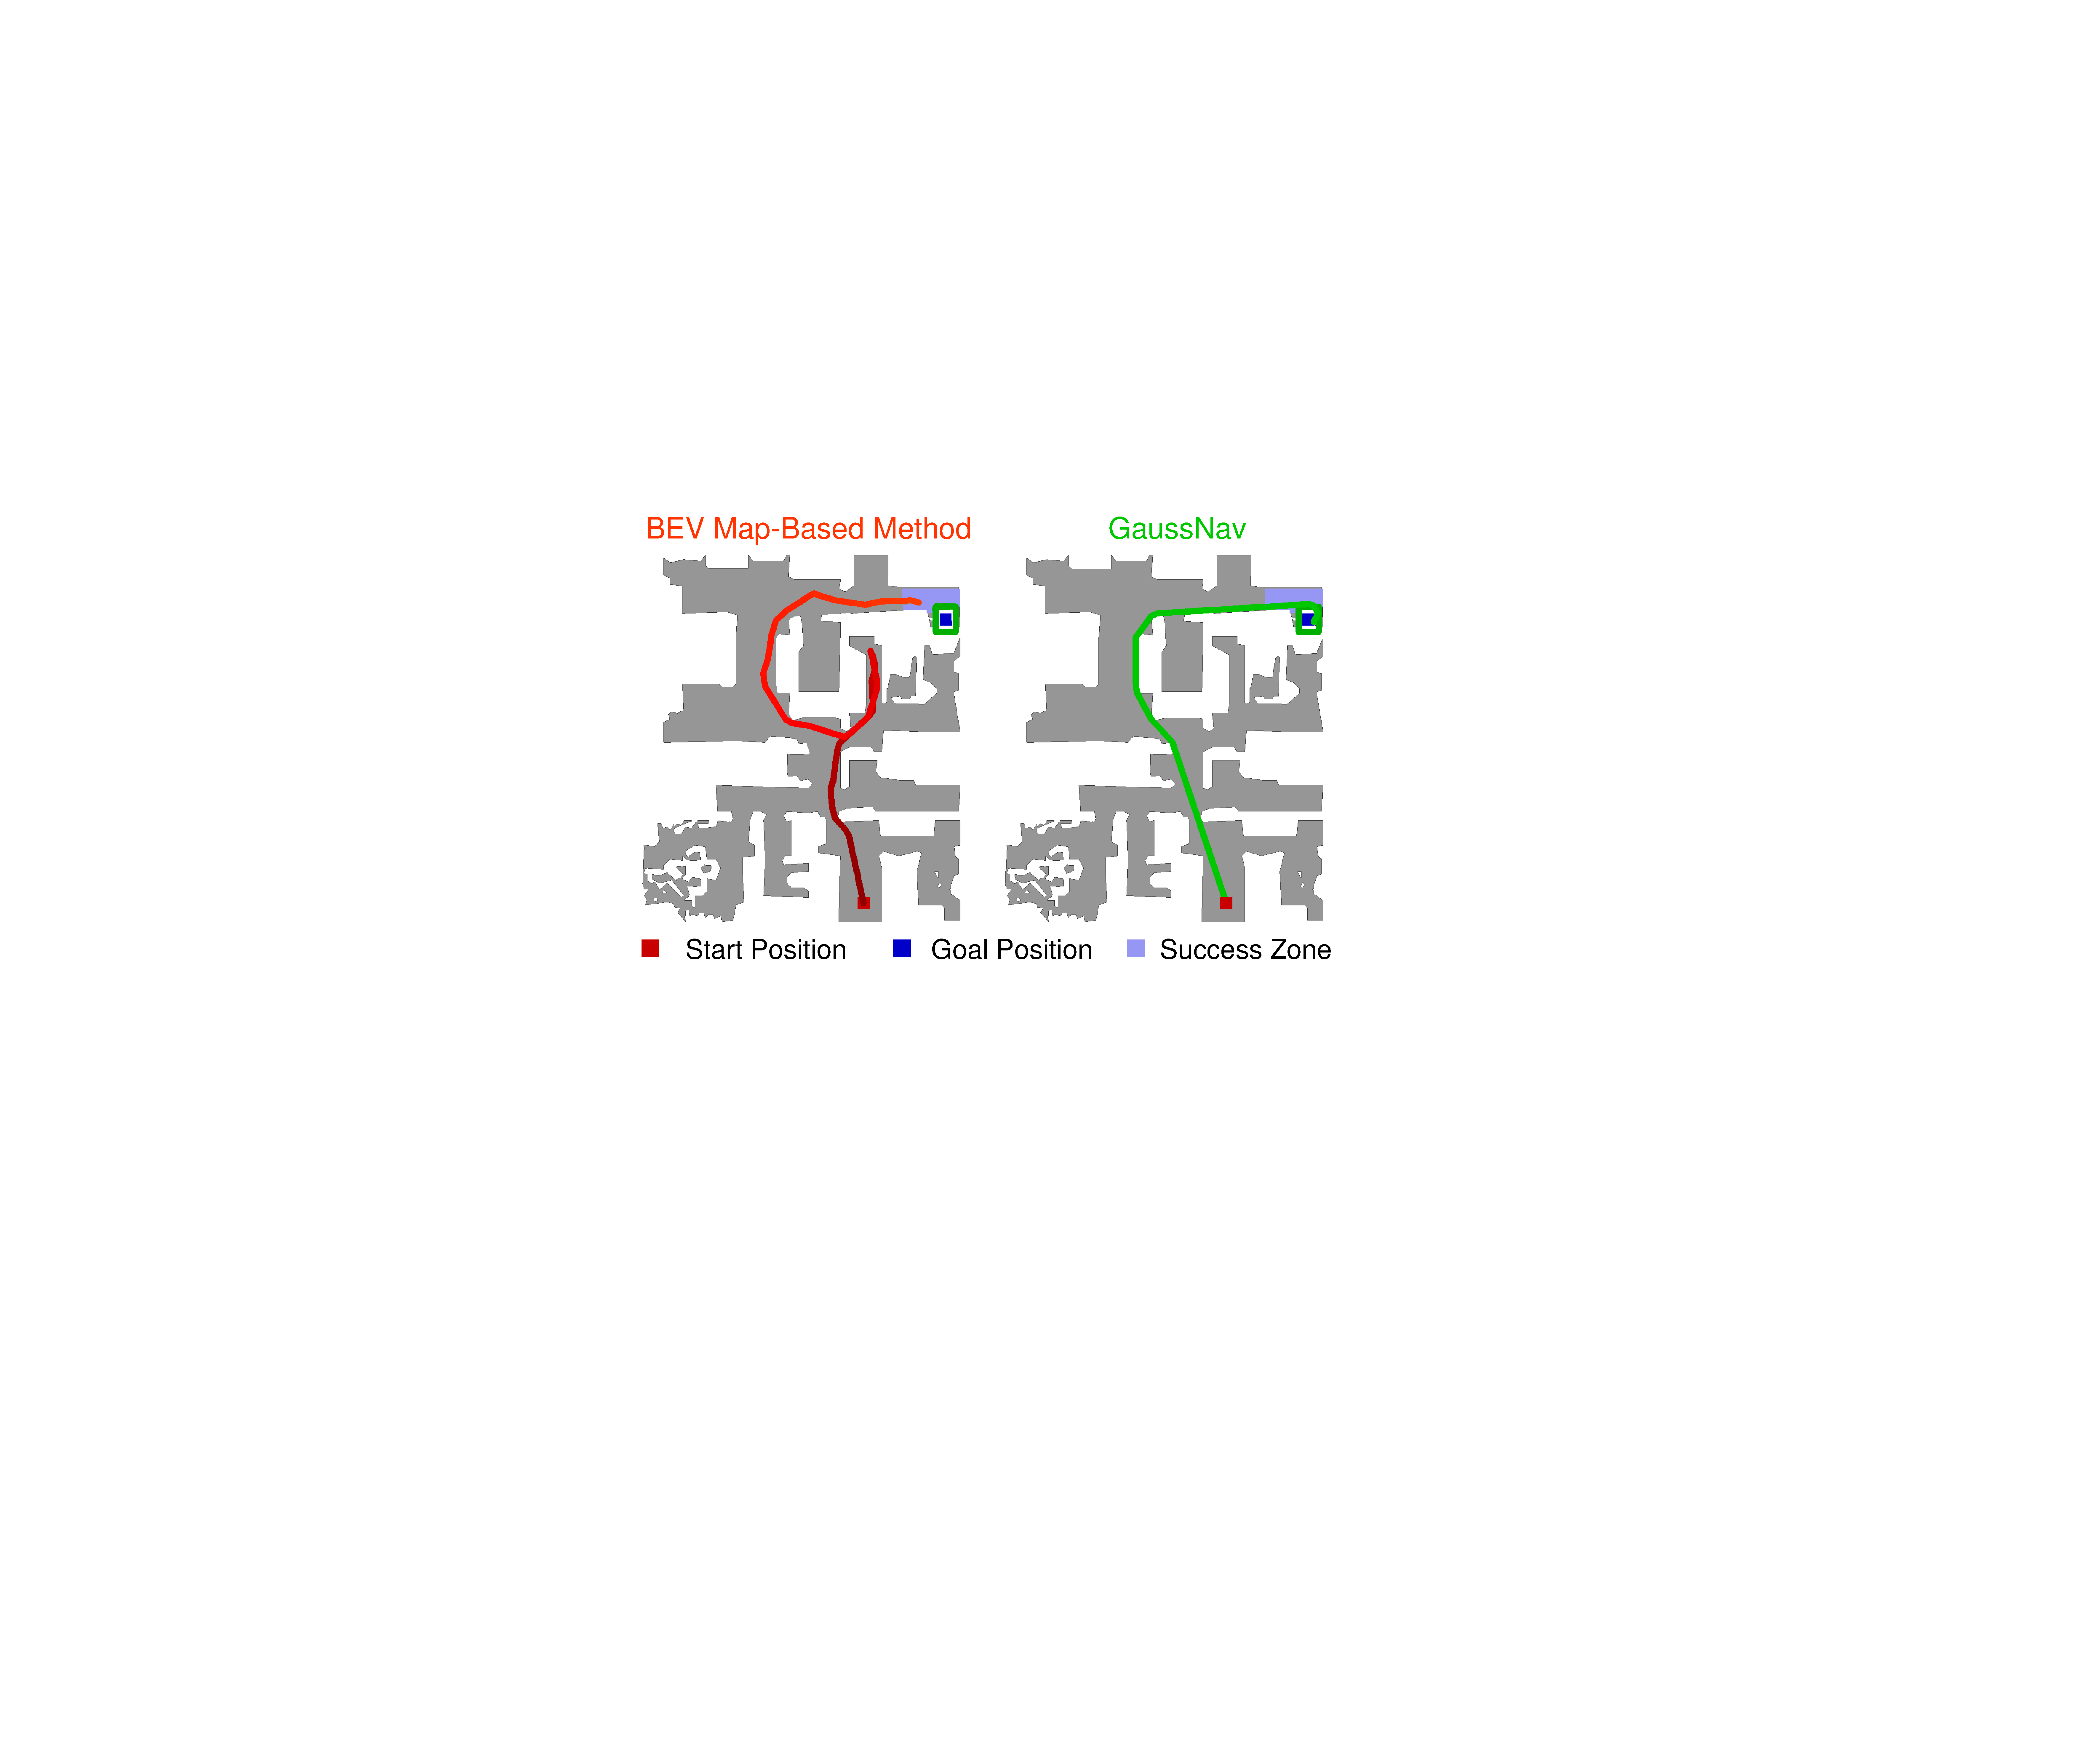
\includegraphics[width=0.45\textwidth]{pics/trajectory.pdf}
\caption{轨迹分析。我们的语义高斯地图表示使智能体能够从单张目标图像直接定位目标物体，从而实现高效的视觉导航。}
\label{fig:trajectory}
\vspace{-10pt}
\end{figure}

\textbf{动作空间。} 我们使用离散动作空间进行导航，包含四个动作：\{\texttt{停止(STOP)}, \texttt{前进(FORWARD)}, \texttt{右转(TURN\_RIGHT)}, \texttt{左转(TURN\_LEFT)}\}。\texttt{停止}动作终止当前回合，\texttt{前进}动作使智能体向前移动25厘米。旋转动作在原地执行：\texttt{右转}产生25度顺时针旋转，\texttt{左转}产生25度逆时针旋转。

\textbf{评估指标。} 遵循Krantz等人\cite{krantz2022instancespecific}的方法，我们从成功率和效率两个方面评估模型。我们报告成功率(Success)和归一化逆路径长度加权成功率(SPL)。如果智能体在距离目标物体1.0米的欧氏距离内调用\texttt{停止}动作，则该回合被判定为成功（$\text{Success} = 1$）。SPL是文献\cite{anderson2018evaluation}中定义的效率指标，计算公式为：
\begin{equation}
    \text{SPL} = \frac{1}{N} \sum_{i=1}^{N} S_i \cdot \frac{l_i}{\max(p_i, l_i)},
\end{equation}
其中$N$是总回合数，$S_i$是第$i$个回合的二元成功指示符，$l_i$是从起始位置到目标的最短路径距离，$p_i$是智能体实际走过的路径长度。SPL值越高表示导航效率越高。



\subsection{与当前最优方法的对比}

我们将所提模型与各种基线方法和先前的最优工作进行了评估对比，结果如\Cref{tab:main}所示。与传统的IIN方法为每个回合生成一张地图不同，GaussNav在一个场景的多个回合之间构建统一的地图。第一部分列出了端到端基线方法的结果，第二部分包括为MultiON任务设计但在此处用于IIN任务的方法。\Cref{tab:main}的第三部分展示了原始IIN最优方法的性能，第四部分报告了这些方法在适配使用场景地图后的性能。

\textbf{端到端基线方法。} 我们评估了两种端到端方法在IIN任务上的性能。\textit{RL基线}构建了一个网络，输入包括智能体RGB图像$(\mathcal{V}_{RGB})$、智能体深度图像$(\mathcal{V}_{D})$、目标图像$(\mathcal{V}_G)$、GPS坐标$(x,z)$和航向角$(\theta)$。视觉观测使用独立的ResNet-18\cite{he2016deep}编码器进行编码，GPS和航向角使用32维线性层进行编码。然后将这些特征拼接起来，通过一个2层LSTM进行编码。最后，从类别分布中采样动作$a(t)$。该网络使用近端策略优化(PPO)\cite{schulman2017proximal}从头开始训练。

Yadav等人\cite{yadav2023ovrl}提出的\textit{OVRL-v2}为图像目标导航中的视觉编码器引入了自监督预训练。OVRL-v2最初是为图像目标导航任务训练的。直接将OVRL-v2应用于IIN任务而不进行微调会导致性能不佳，成功率仅为0.006（\Cref{tab:main}第2行）。这种性能下降可归因于多个因素：场景数据集从Gibson\cite{xia2018gibson}切换到HM3D\cite{yadav2023habitat}、机器人形态从Locobot\footnote{\url{http://www.locobot.org/}}变为Stretch，以及目标目的地的性质从图像来源变为图像主体。在HM3D数据集上针对IIN任务专门微调OVRL-v2后，性能显著提升，成功率达到0.248（\Cref{tab:main}第3行）。


\textbf{MultiON任务中的最优方法。} MultiON任务与我们评估GaussNav时使用的场景特定地图表示有许多相似之处。我们在IIN基准上重新实现了几种MultiON任务的最优方法\cite{wani2020multion, chen2022learning, marza2023multi}。值得注意的是，我们直接将目标物体的语义类别输入到上述方法中。由于IIN任务的导航要求是实例级而非语义级的，这种任务表述上的差异为性能提升留下了空间。

\begin{table}[tb]
  \centering
  % Increase the padding of the columns
  % \setlength{\tabcolsep}{16pt}
  % Optionally, use a smaller font for the table
  \small
  \begin{tabular}{@{}l c c@{}}
    \toprule
    Ablations & Success~$\uparrow$ & SPL~$\uparrow$ \\
    \midrule
    GaussNav & 0.725 & 0.578  \\
    GaussNav w.o. Classifier & 0.375 & 0.291 \\
    GaussNav w.o. Match & 0.444 & 0.353 \\
    GaussNav w.o. NVS & 0.716 & 0.557 \\
    GaussNav w. SIFT & 0.655 & 0.519 \\
    GaussNav w. GlueStick \cite{pautrat_suarez_2023_gluestick} & 0.723 & 0.577 \\
    GaussNav w. GT Match & 0.850 & 0.672 \\ 
    GaussNav w. GT Goal Localization & 0.946 & 0.744 \\
    \bottomrule
  \end{tabular}
  % \vspace{-10pt}
  \vspace{5pt}
  \caption{Ablation study of GaussNav. We study the impact of Classifier, Match module, novel view synthesis (NVS) and different local feature extraction and matching algorithms on our GaussNav. The last two rows describe the performance of our method using ground truth match results and goal position.}  
  \vspace{-14pt}
  \label{tab:ablations}
\end{table}

% \begin{table*}[tb]
%     \centering
%     % \begin{tabular}{|l|c|c|c|c|c|c|c|}
%     % \small
%     \begin{tabular}{lcccccccc}
%         \hline
%         Method & Metric & Chair & Sofa & Plant & Bed & Toilet & TV & Total \\
%         \hline
%         \multirow{2}{*}{\textbf{w.o.} classifier} & Success $\uparrow$ & \textbf{0.821} & \textbf{0.873} & 0.798 & \textbf{0.914} & \textbf{0.936} & 0.829 & \textbf{0.840} \\
%         \cline{2-9}
%         & Time (s) $\downarrow$ & 30.9 & 24.8 & 33.2 & 18.1 & 24.6 & 31.9 & 29.0 \\
%         \hline
%         \multirow{2}{*}{\textbf{w}. classifier} & Success $\uparrow$ & 0.782 & 0.859 & \textbf{0.854} & 0.878 & 0.702 & \textbf{0.847} & 0.811 \\
%         \cline{2-9}
%         & Time (s) $\downarrow$ & \textbf{15.7} & \textbf{8.09} & \textbf{11.6} & \textbf{5.97} & \textbf{1.85} & \textbf{2.74} & \textbf{11.5}  \\
%         \hline
%     \end{tabular}
%     \caption{Results of matching success and time taken with or without classifier.}
%     \vspace{-12pt}
%     \label{tab:abla_classifier}
% \end{table*}

% \begin{table}[tb]
%     \centering
%     \small % Reduce font size
%     \setlength{\tabcolsep}{3pt} % Adjust column spacing (default is 6pt)
%     \begin{tabular}{lccccccc}
%         \hline
%         Method & Metric & Ch. & So. & Pl. & Bed & Tol. & TV \\
%         \hline
%         \multirow{2}{*}{\textbf{w.o.} clf} & Success $\uparrow$ & \textbf{0.821} & \textbf{0.873} & 0.798 & \textbf{0.914} & \textbf{0.936} & 0.829 \\
%         \cline{2-8}
%         & Time (s) $\downarrow$ & 30.9 & 24.8 & 33.2 & 18.1 & 24.6 & 31.9 \\
%         \hline
%         \multirow{2}{*}{\textbf{w}. clf} & Success $\uparrow$ & 0.782 & 0.859 & \textbf{0.854} & 0.878 & 0.702 & \textbf{0.847} \\
%         \cline{2-8}
%         & Time (s) $\downarrow$ & \textbf{15.7} & \textbf{8.09} & \textbf{11.6} & \textbf{5.97} & \textbf{1.85} & \textbf{2.74}  \\
%         \hline
%     \end{tabular}
%     \caption{Results of matching success and time taken with or without classifier.}
%     \label{tab:abla_classifier}
% \end{table}

\begin{table}[tb]
    \centering
    \small % Reduce font size
    \renewcommand{\arraystretch}{1.2} % Adjust row spacing (default is 1.0)
    \setlength{\tabcolsep}{3pt} % Adjust column spacing (default is 6pt)
    \begin{tabular}{lccccccc}
        \hline
        Method & Metric & Ch. & So. & Pl. & Bed & Tol. & TV \\
        \hline
        \multirow{2}{*}{\textbf{w.o.} clf} & Success $\uparrow$ & \textbf{0.821} & \textbf{0.873} & 0.798 & \textbf{0.914} & \textbf{0.936} & 0.829 \\
        \cline{2-8}
        & Time (s) $\downarrow$ & 30.9 & 24.8 & 33.2 & 18.1 & 24.6 & 31.9 \\
        \hline
        \multirow{2}{*}{\textbf{w}. clf} & Success $\uparrow$ & 0.782 & 0.859 & \textbf{0.854} & 0.878 & 0.702 & \textbf{0.847} \\
        \cline{2-8}
        & Time (s) $\downarrow$ & \textbf{15.7} & \textbf{8.09} & \textbf{11.6} & \textbf{5.97} & \textbf{1.85} & \textbf{2.74}  \\
        \hline
    \end{tabular}
    \vspace{5pt}
    \caption{Results of matching success and time taken with or without classifier.(Abbreviations: clf = classifier, Ch. = Chair, So. = Sofa, Pl. = Plant, Tol. = Toilet)}
    \vspace{-24pt}
    \label{tab:abla_classifier}
\end{table}

% \begin{table*}[b] % The [b] option places the table at the bottom of the page
%     \centering
%     \begin{tabular}{lcccccccc}
%         \hline
%         Method & Metric & Chair & Sofa & Plant & Bed & Toilet & TV & Total \\
%         \hline
%         \multirow{2}{*}{\textbf{w.o.} classifier} & Success $\uparrow$ & \textbf{0.821} & \textbf{0.873} & 0.798 & \textbf{0.914} & \textbf{0.936} & 0.829 & \textbf{0.840} \\
%         \cline{2-9}
%         & Time (s) $\downarrow$ & 30.9 & 24.8 & 33.2 & 18.1 & 24.6 & 31.9 & 29.0 \\
%         \hline
%         \multirow{2}{*}{\textbf{w}. classifier} & Success $\uparrow$ & 0.782 & 0.859 & \textbf{0.854} & 0.878 & 0.702 & \textbf{0.847} & 0.811 \\
%         \cline{2-9}
%         & Time (s) $\downarrow$ & \textbf{15.7} & \textbf{8.09} & \textbf{11.6} & \textbf{5.97} & \textbf{1.85} & \textbf{2.74} & \textbf{11.5}  \\
%         \hline
%     \end{tabular}
%     \caption{Results of matching success and time taken with or without classifier.}
%     \label{tab:abla_classifier}
% \end{table*}



\textbf{IIN任务中的最优方法。} 为了进行公平对比，我们使用两种地图表示（回合地图和场景特定地图）评估了先前IIN最优方法\cite{krantz2023navigating, lei2024instanceaware}的性能。\textit{Mod-IIN}\cite{krantz2023navigating}将IIN任务分解为探索、目标实例重识别、目标定位和局部导航。该方法利用特征匹配在以自我为中心的视觉中重新识别目标实例，并将匹配的特征投影到地图上以定位目标。每个子任务都使用无需微调的现成组件解决。

\textit{IEVE}\cite{lei2024instanceaware}采用模块化架构，能够在探索、验证和利用动作之间动态切换。这种灵活性使智能体能够根据不同情况做出明智的决策。\textit{Mod-IIN}和\textit{IEVE}在IIN任务上都表现出了出色的性能。我们还在这些方法中实现了场景特定地图表示，以便与GaussNav进行公平对比。如\Cref{tab:main}所示，GaussNav在所有方法中都表现出显著的性能优势。它在SPL指标上以0.231的巨大幅度超越了所有现有模型（最后两行）。这一结果表明，我们的语义高斯地图通过保留场景中物体的精细纹理细节，使智能体能够基于目标图像直接定位目标物体，而无需额外的验证步骤。


我们将这种卓越的性能归因于语义高斯这一新颖的地图表示，它使智能体无需额外的探索或验证即可直接定位目标，如\Cref{fig:trajectory}所示。与之前广泛使用的BEV地图表示不同，我们的语义高斯地图允许智能体通过语义标签输入查询高斯，并渲染物体实例的描述性图像。因此，与基于BEV地图的方法不同，我们的GaussNav不需要对潜在的物体候选进行显式验证。相反，它从众多可能性中选择最可能的候选，并直接向其导航。

\begin{figure}[tb]
\centering
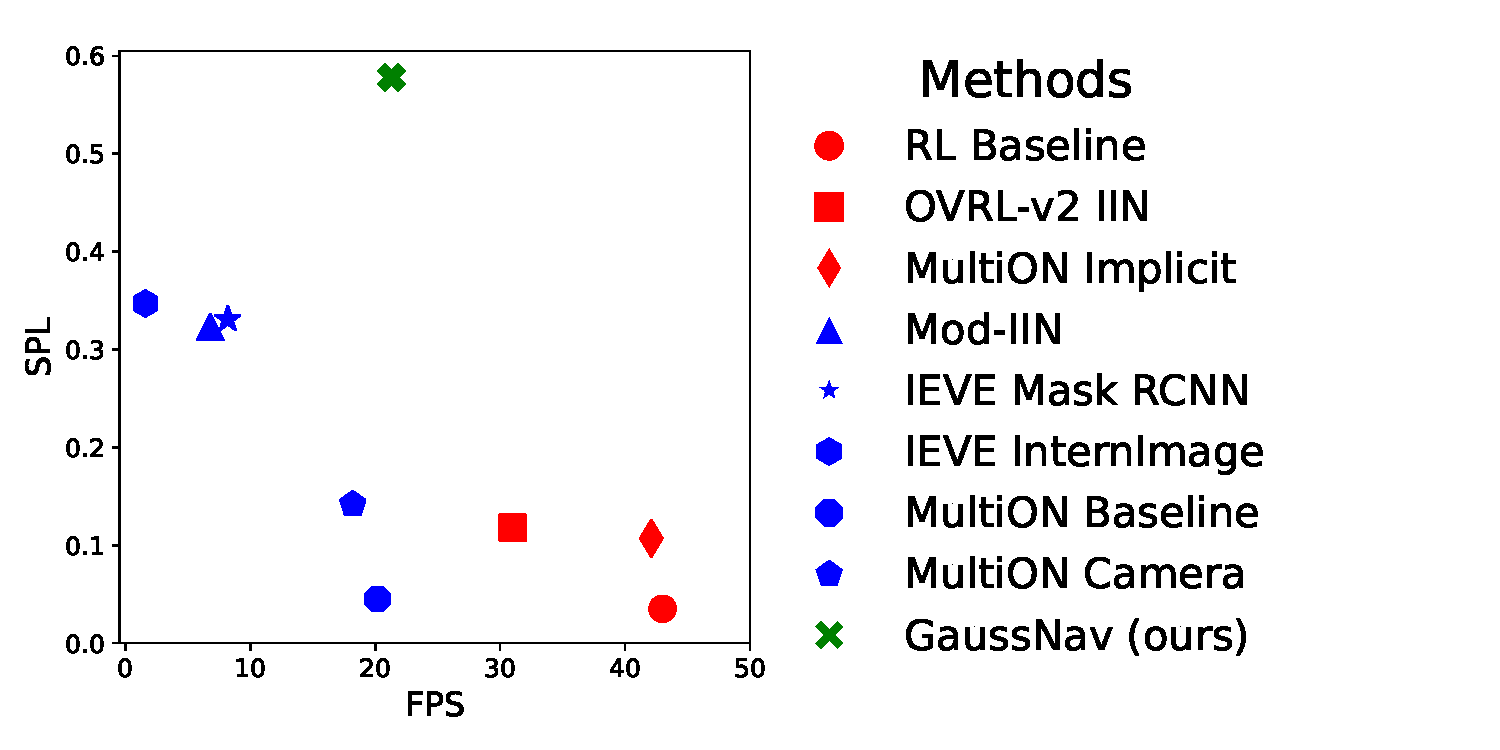
\includegraphics[width=0.45\textwidth]{pics/framerate.pdf}
\caption{SPL和帧率分析。{\color{red}红色标记}代表端到端方法，{\color{blue}蓝色标记}代表模块化方法。我们的{\color{MyGreen}GaussNav}属于模块化方法，在模块化方法中实现了最高的帧率，同时在所有IIN任务方法中取得了最高的SPL。}
\vspace{-10pt}
\label{fig:framerate}
\end{figure}


\begin{figure*}
  \centering
  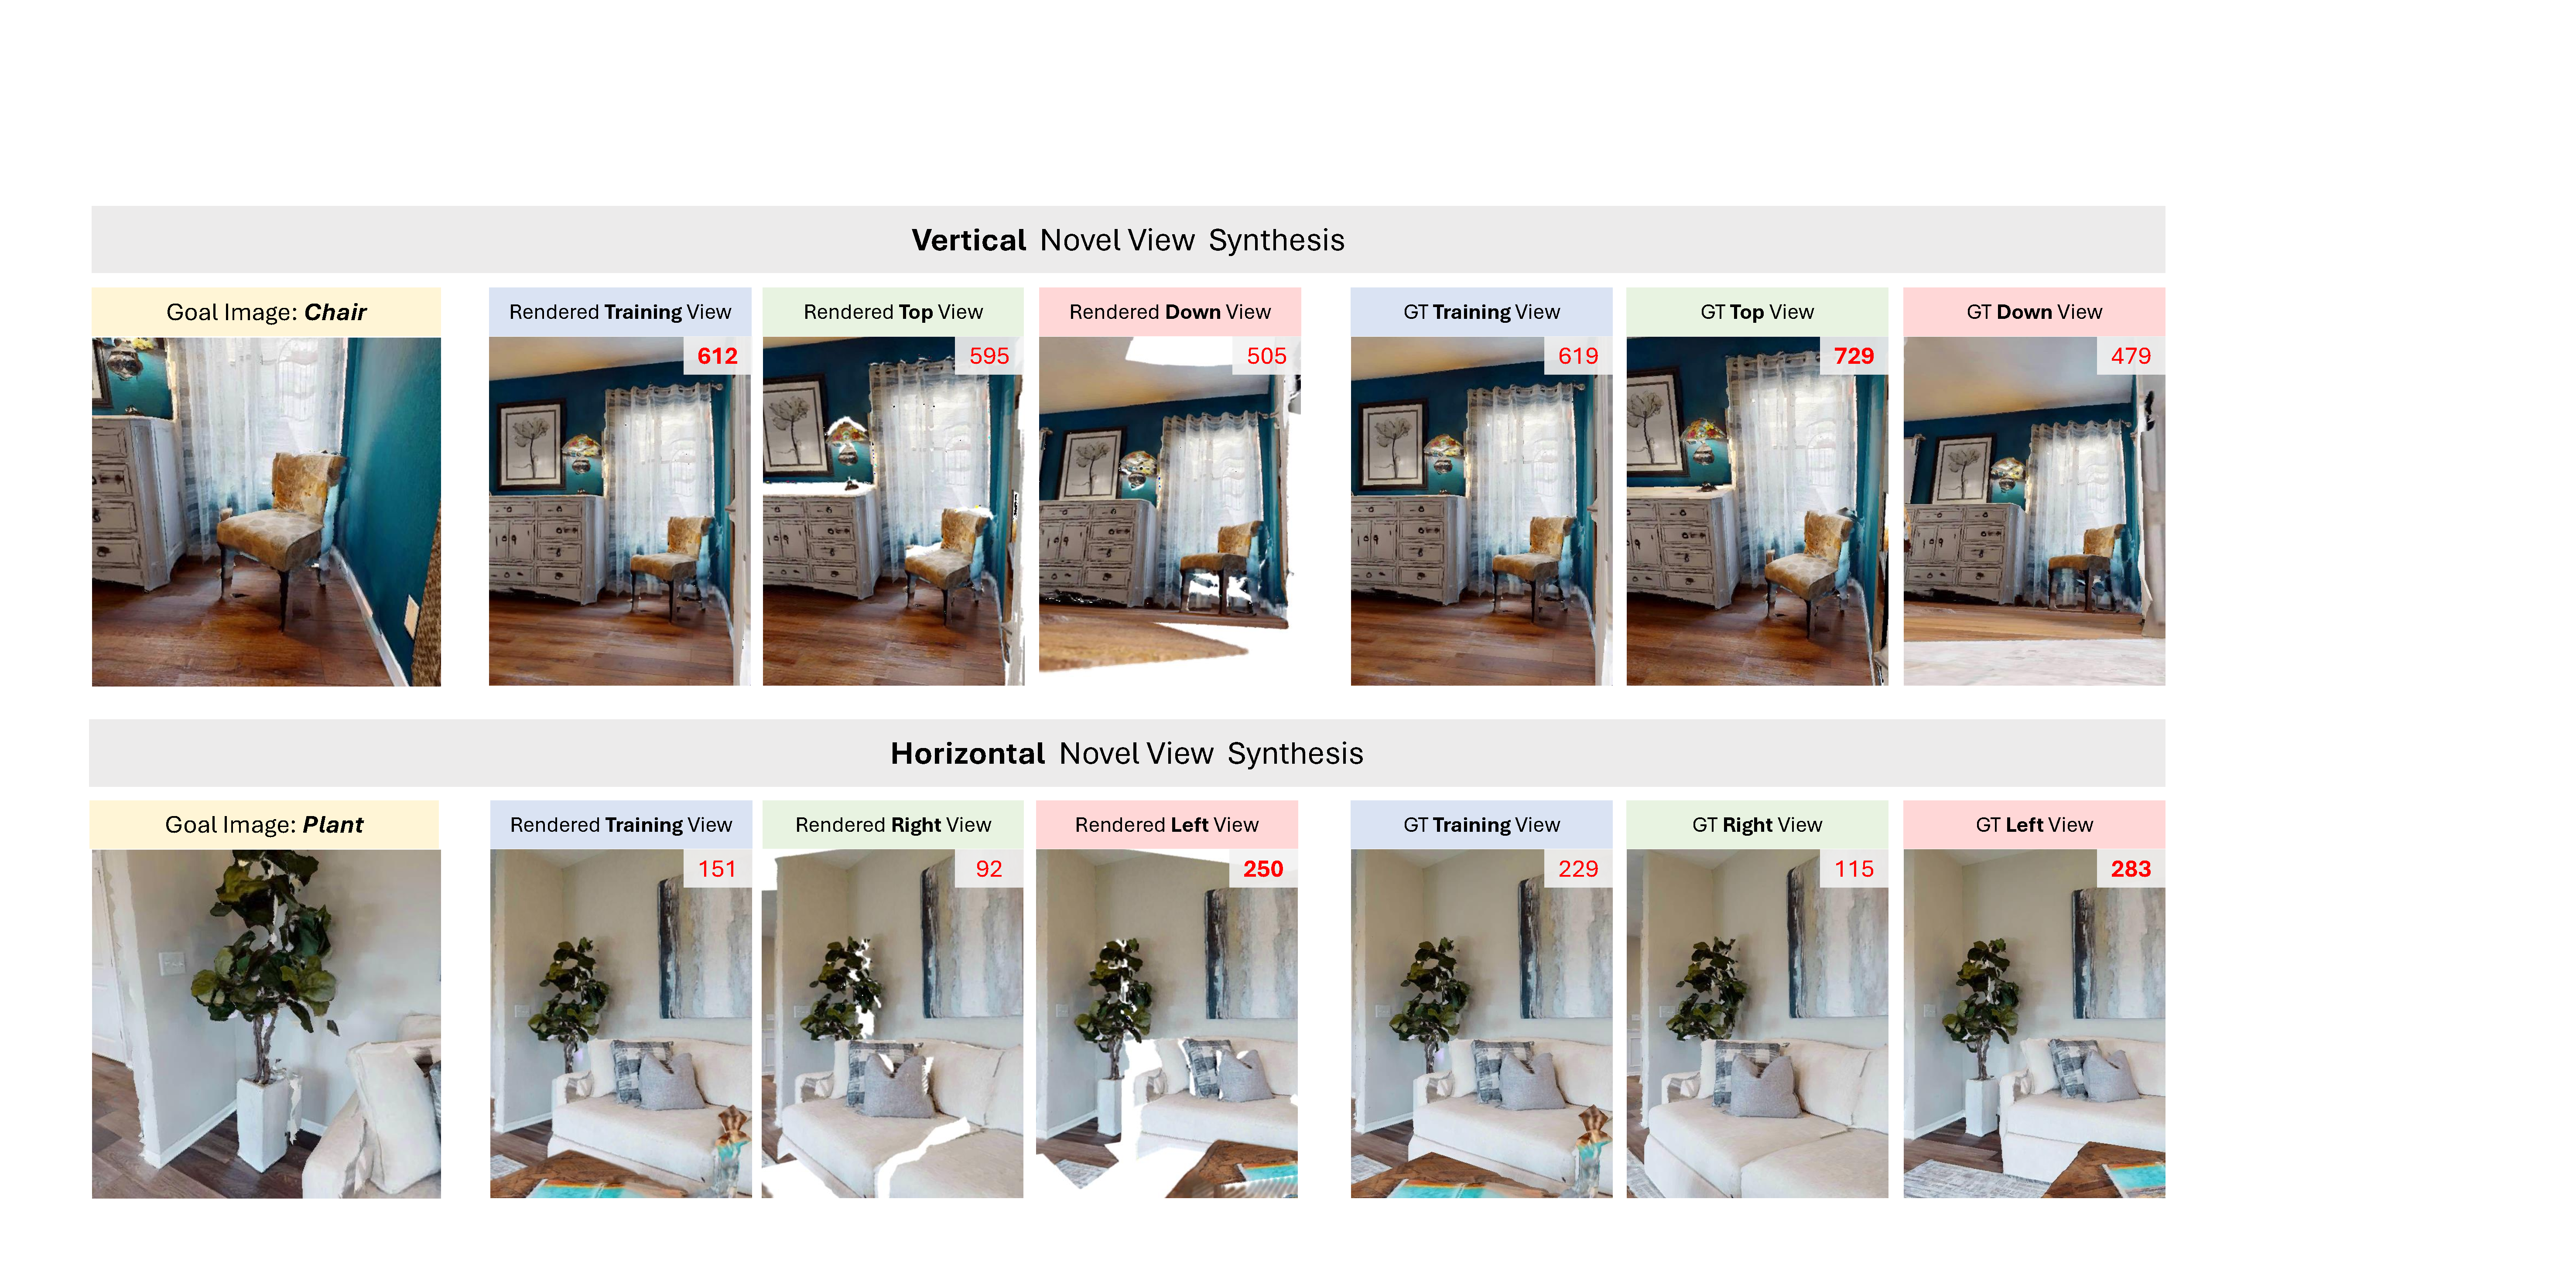
\includegraphics[width=0.95\linewidth]{pics/NVS.pdf}
  \vspace{-10pt}
  \caption{新视角合成结果可视化。可视化结果包括$\theta = \pm15^\circ$的水平和垂直新视角合成结果。每张图像的右上角显示了与目标图像匹配的关键点数量。
  }
  \vspace{-6pt}
  \label{fig:NVS}
\end{figure*}

\begin{table}[tb]
  \centering
  % Increase the padding of the columns
  % \setlength{\tabcolsep}{16pt}
  % Optionally, use a smaller font for the table
  \small
  % \vspace{-18pt}
  \vspace{6pt}
  \begin{tabular}{@{}c c c c c c@{}}
    \toprule
    Chair & Sofa & TV & Plant & Toilet & Bed \\
    \midrule
    11 & 2 & 1 & 3 & 1 & 0 \\
    \bottomrule
  \end{tabular}
  % \vspace{-10pt}
  \vspace{5pt}
  \caption{Number of object instances across different categories in the first floor of scene \texttt{CrMo8WxCyVb}.} 
  \vspace{-24pt}
  \label{tab:time}
\end{table}

\begin{table*}[tb]
    \renewcommand{\arraystretch}{1.2} % Increase the row height
    \centering
    \begin{tabular}{c cc cc cc cc cc}
        \hline
        \multirow{2}{*}{Metric} & original & GT original & \multicolumn{2}{c}{horizontal} & \multicolumn{2}{c}{vertical} & \multicolumn{2}{c}{GT horizontal} & \multicolumn{2}{c}{GT vertical} \\
        \cline{2-11}
        & $n_v=1$ & $n_v=1$ & $n_v=3$ & $n_v=5$ & $n_v=3$ & $n_v=5$ & $n_v=3$ & $n_v=5$ & $n_v=3$ & $n_v=5$ \\
        \hline
        Success $\uparrow$ & 0.811 & 0.815 & 0.824 & 0.827 & 0.832 & 0.831 & 0.835 & 0.846 & 0.839 & 0.845 \\
        Time (s) $\downarrow$ & 11.5 & 11.7 & 32.1 & 53.9 & 33.1 & 54.2 & 32.7 & 54.1 & 33.4 & 55.1 \\
        \hline
    \end{tabular}
    \vspace{5pt}
    \caption{Results of the number of rendered images $n$, different directions (vertical or horizontal) and whether to use ground truth rendering's impact on the matching success.}
    \vspace{-16pt}
    \label{tab:NVS}
\end{table*}

% \begin{table*}[tb]
%     \centering
%     \begin{tabularx}{\textwidth}{>{\raggedright\arraybackslash}p{2cm}*{10}{>{\centering\arraybackslash}X}}
%         \hline
%         \multirow{2}{*}{Metric} & o. & GT o. & \multicolumn{2}{c}{hor.} & \multicolumn{2}{c}{ver.} & \multicolumn{2}{c}{GT hor.} & \multicolumn{2}{c}{GT ver.} \\
%         \cline{2-11}
%         & $n_v=1$ & $n_v=1$ & $n_v=3$ & $n_v=5$ & $n_v=3$ & $n_v=5$ & $n_v=3$ & $n_v=5$ & $n_v=3$ & $n_v=5$ \\
%         \hline
%         Success $\uparrow$ & 0.811 & 0.815 & 0.824 & 0.827 & 0.832 & 0.831 & 0.835 & 0.846 & 0.839 & 0.845 \\
%         Time (s) $\downarrow$ & 11.5 & 11.7 & 32.1 & 53.9 & 33.1 & 54.2 & 32.7 & 54.1 & 33.4 & 55.1 \\
%         \hline
%     \end{tabularx}
%     \caption{Results of the number of rendered images $n$, different directions (ver. or hor.) and the impact of using ground truth rendering on matching success. The o.\ means the original training view, \textit{hor.} indicates horizontal NVS, and \textit{ver.} represents vertical NVS. $n$ is the number of rendered images.}
%     \label{tab:NVS}
% \end{table*}

% \begin{table*}[tb]
%     \renewcommand{\arraystretch}{1.2} % Increase the row height
%     \centering
%     % \large % Increase the font size within the table
%     \begin{tabularx}{\textwidth}{>{\raggedright\arraybackslash}p{2.5cm}*{10}{>{\centering\arraybackslash}X}}
%         \hline
%         \multirow{2}{*}{Metric} & o. & GT o. & \multicolumn{2}{c}{hor.} & \multicolumn{2}{c}{ver.} & \multicolumn{2}{c}{GT hor.} & \multicolumn{2}{c}{GT ver.} \\
%         \cline{2-11}
%         & $n_v=1$ & $n_v=1$ & $n_v=3$ & $n_v=5$ & $n_v=3$ & $n_v=5$ & $n_v=3$ & $n_v=5$ & $n_v=3$ & $n_v=5$ \\
%         \hline
%         Success $\uparrow$ & 0.811 & 0.815 & 0.824 & 0.827 & 0.832 & 0.831 & 0.835 & 0.846 & 0.839 & 0.845 \\
%         Time (s) $\downarrow$ & 11.5 & 11.7 & 32.1 & 53.9 & 33.1 & 54.2 & 32.7 & 54.1 & 33.4 & 55.1 \\
%         \hline
%     \end{tabularx}
%     \caption{Results of the number of rendered images $n$, different directions (ver.\ or hor.), and the impact of using ground truth rendering on matching success. The o.\ means the original training view, \textit{hor.} indicates horizontal NVS, and \textit{ver.} represents vertical NVS. $n$ is the number of rendered images.}
%     \label{tab:NVS}
% \end{table*}



\subsection{消融实验}

为了理解GaussNav各个模块的作用，我们进行了以下消融实验：

\textbf{移除分类器的GaussNav。} 在\Cref{fig:main}中，我们将分类器的输出替换为随机生成的目标类别。我们观察到成功率下降到0.375，SPL下降到0.291（\Cref{tab:ablations}第2行）。为了更好地评估分类器，我们设计了以下实验。我们将来自所有候选物体的训练视图定义为全集，将经过分类器过滤的训练视图定义为子集。给定目标图像和关键点匹配器，我们分别在每个集合中计算匹配关键点数量最多的视图。如果该视图包含目标物体，则视为成功；否则视为失败。我们还记录了整个局部特征匹配过程所花费的总时间，以评估分类器对效率的影响。这里我们不使用成功率和SPL等导航指标，因为这样可以消除路径规划错误等无关因素的影响。实验结果如\Cref{tab:abla_classifier}所示。可以看出，没有分类器时的总成功率略高于有分类器时（提高了0.039），但提升有限。然而，所花费的时间是有分类器时的2.5倍，效率显著降低。因此，考虑到性能和效率之间的权衡，我们选择将分类器作为GaussNav框架的一个组件。


% 这是因为正确分类是我们的方法过滤潜在候选的前提。

\textbf{移除匹配模块的GaussNav。} 匹配模块旨在从同类别候选中区分出目标。没有匹配模块时，我们从这些候选中随机选择。成功率和SPL分别下降到0.444和0.353（\Cref{tab:ablations}第3行）。这可归因于没有匹配模块时对候选实例的随机选择。

\textbf{使用SIFT或GlueStick的GaussNav。} 为了评估不同的特征提取器和匹配算法对GaussNav的影响，我们替换了DISK\cite{tyszkiewicz2020disk}+LightGlue\cite{lindenberger2023lightglue}组合。我们使用SIFT+FLANN和GlueStick\cite{pautrat_suarez_2023_gluestick}作为替代方案。第一种替换导致性能下降较大（\Cref{tab:ablations}第4行），第二种仅显示出轻微下降（\Cref{tab:ablations}第5行）。这些结果表明，不同的局部特征匹配算法在HM3D数据集上表现出不同的性能。

\textbf{新视角合成(NVS)分析。} 我们进行实验以评估渲染图像数量$n_v$和NVS上限的影响。具体而言，我们在水平和垂直方向上分别对$n_v=3$和$n_v=5$的NVS进行了消融研究，并评估了使用真实值(GT)渲染结果可达到的上限。为了避免导航中其他因素的影响，我们仅将通过关键点匹配检索到的图像包含目标物体视为成功；否则视为失败。具体的评估指标在\textbf{移除分类器的GaussNav}部分有详细说明。实验结果如\Cref{tab:NVS}所示。总体而言，使用NVS有助于成功识别物体。然而，较大的$n_v$并不一定产生积极效果（见\Cref{tab:NVS}，垂直$n_v=5$与垂直$n_v=3$对比）。这是因为我们的语义高斯地图对于特定物体可能只有少数几个观测视角，而传统3DGS中通常有几十个。因此，从新视角渲染时可能会出现孔洞等伪影，减少了特征数量，如\Cref{fig:NVS}所示。尽管如此，对于真实值NVS，性能提升是显著的。

\begin{table}[tb]
    \centering
    \vspace{5pt}
    \begin{tabular}{l c c c c c}
        \toprule
         Method & Ver. NVS & Hor. NVS & GT & Success~$\uparrow$ & SPL~$\uparrow$  \\
         \midrule
         IEVE~\cite{lei2024instanceaware} & - & - & - & 0.702 & 0.252 \\
         GaussNav (ours) & $\checkmark$ & $\times$ & $\times$ & 0.713 & 0.259 \\
         GaussNav (ours) & $\times$ & $\checkmark$ & $\times$ & 0.715 & 0.261 \\
         GaussNav (ours) & $\checkmark$ & $\checkmark$ & $\times$ & 0.723 & 0.265 \\
         GaussNav (ours) & $\checkmark$ & $\checkmark$ & $\checkmark$ & 0.747 & 0.289 \\
         \bottomrule
    \end{tabular}
    \vspace{-1pt}
    \caption{Performance Comparison of IEVE~\cite{lei2024instanceaware} and GaussNav. We compare GaussNav with the state-of-the-art method IEVE using different map representations. (Abbreviations: Ver. = Vertical, Hor. = Horizontal)}
    \vspace{-30pt}
    \label{tab:pre-exploration}
\end{table}

为了进一步研究无需预探索的NVS的影响，我们采用了与IEVE\cite{lei2024instanceaware}相同的框架，唯一的区别在于地图表示。IEVE使用二维BEV地图，而GaussNav实现了语义高斯地图。此外，GaussNav在每次观测中出现相似物体时都会执行NVS。结果如\Cref{tab:pre-exploration}所示。我们的语义高斯地图在不依赖预探索的情况下增强了现有观测。虽然这种提升可能不如实例级物体定位能力那么显著，但\Cref{tab:pre-exploration}最后一行的结果表明了未来工作的有希望方向。

\subsection{效率分析}

\begin{figure*}
  \centering
  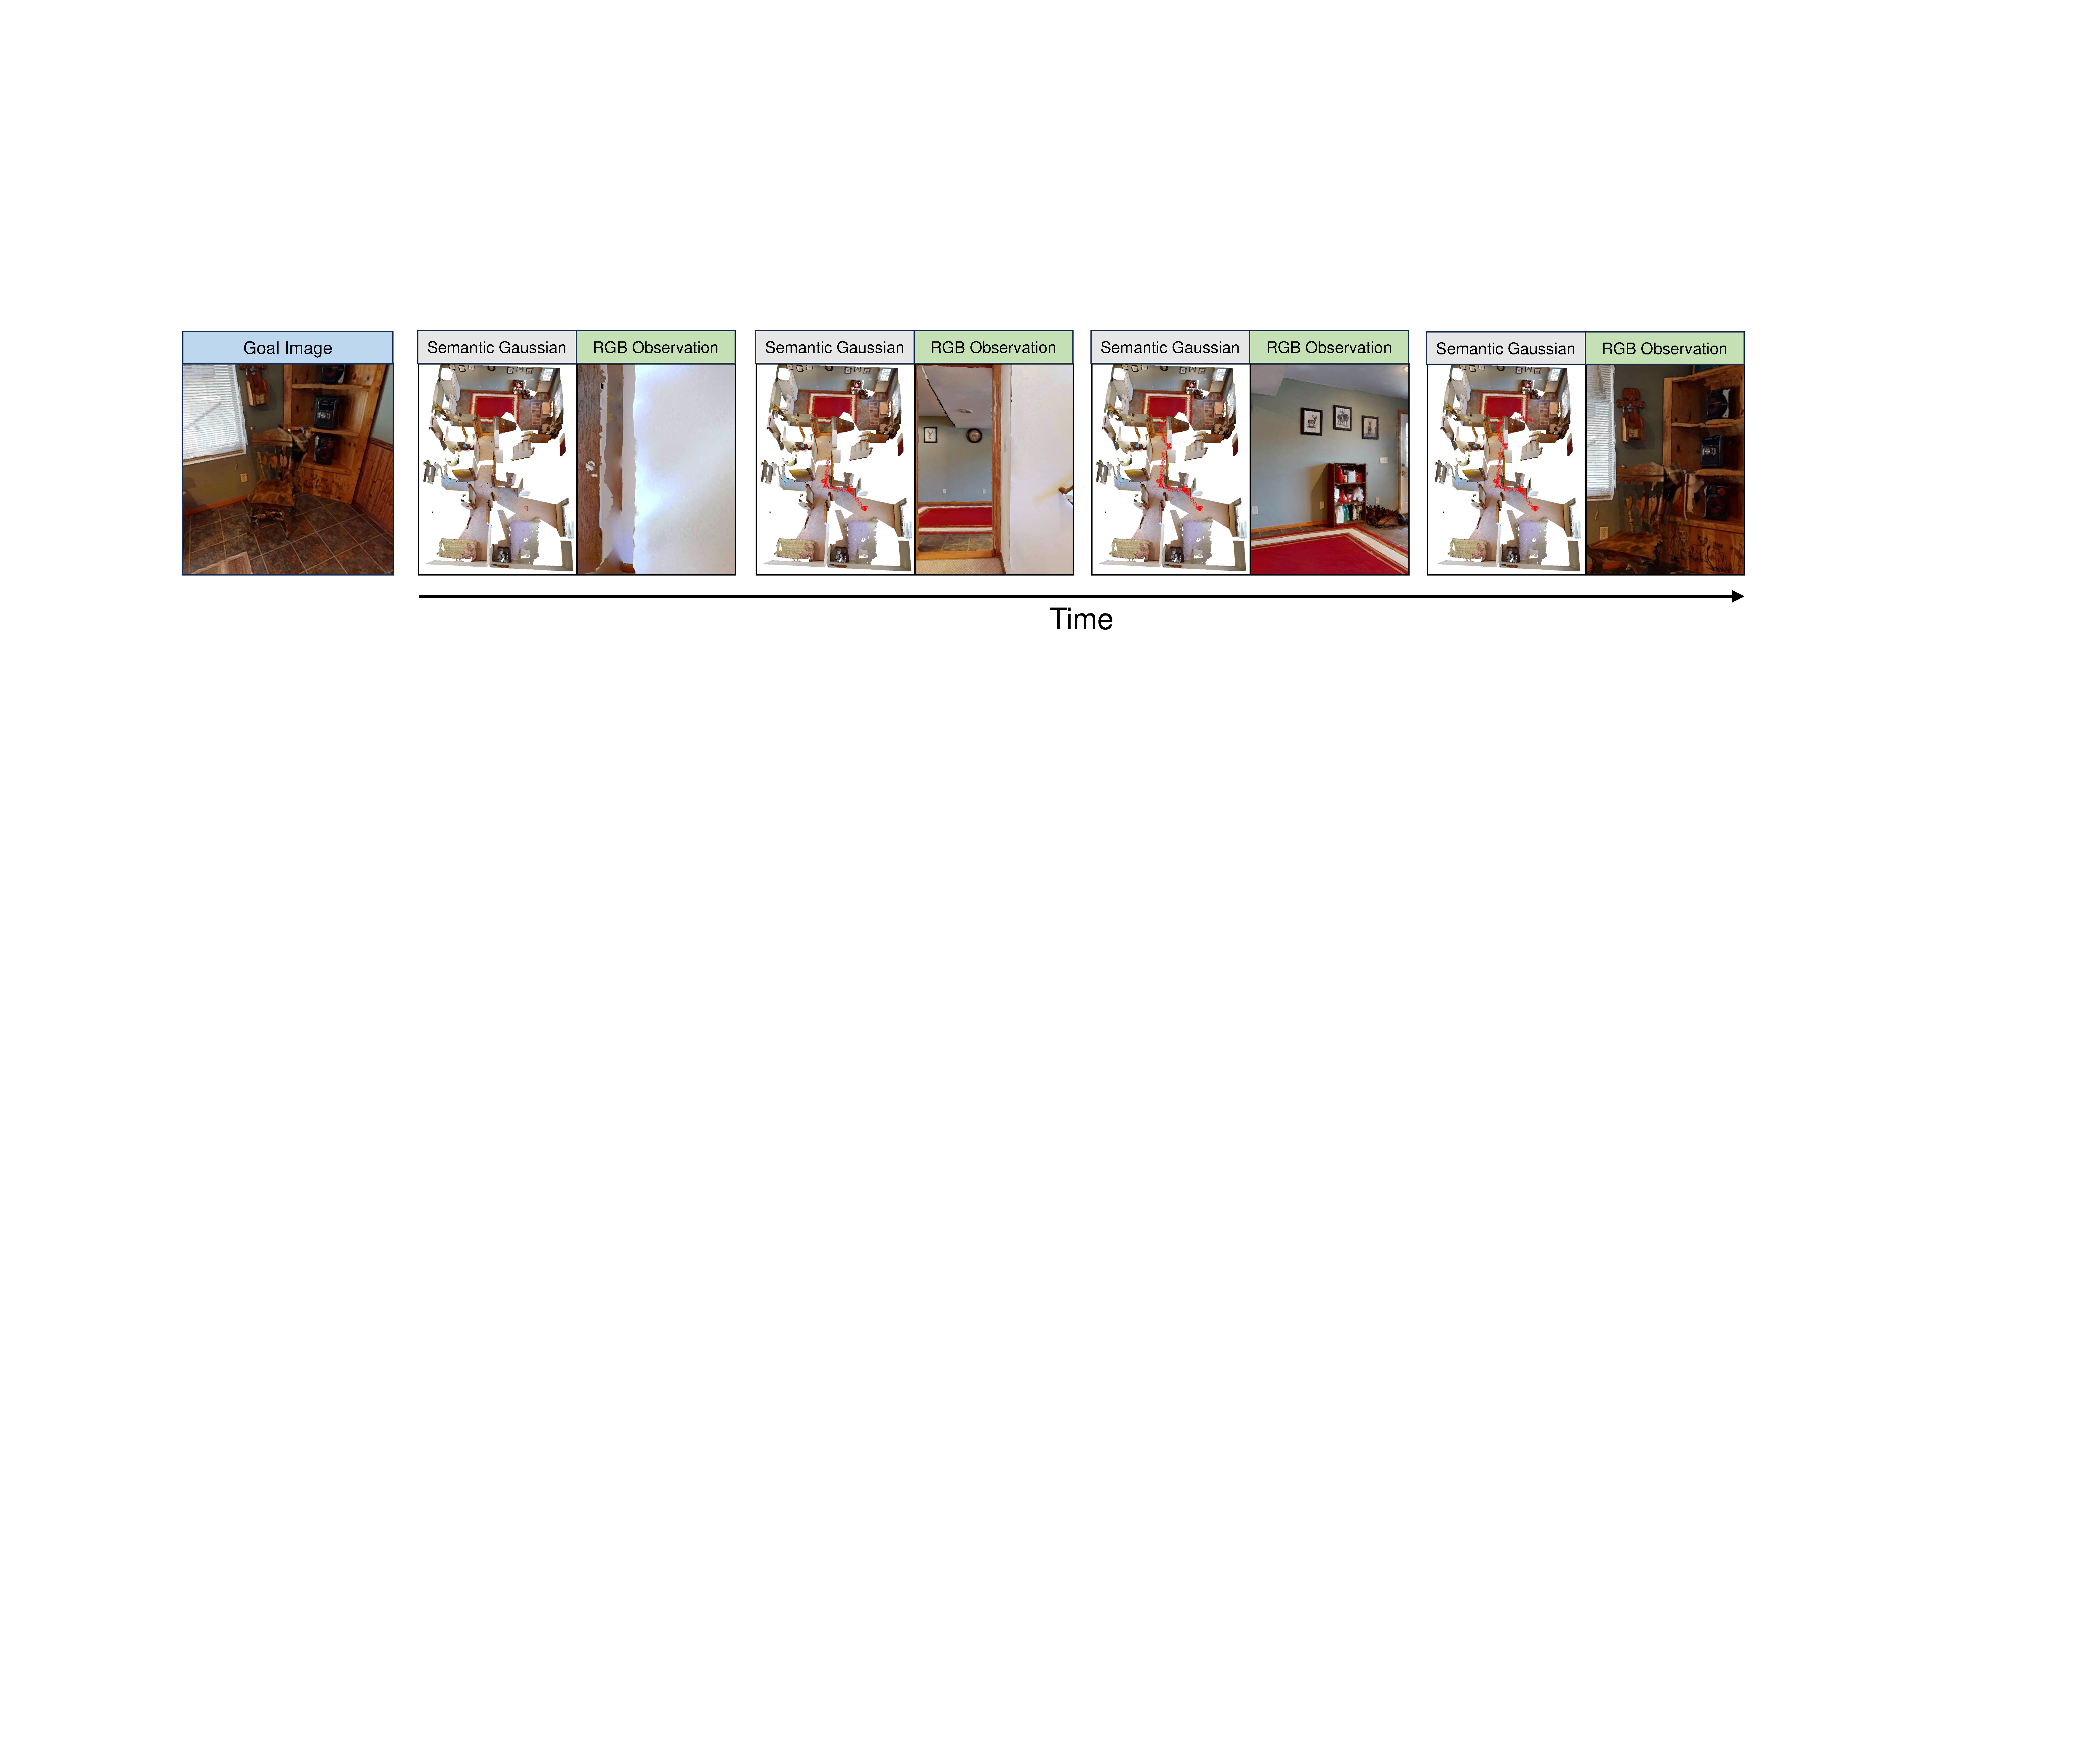
\includegraphics[width=0.95\linewidth]{pics/qualitive_result.pdf}
  \vspace{-10pt}
  \caption{GaussNav智能体在Habitat仿真器中执行IIN任务的定性示例。当在环境中随机初始化时，智能体被提供一张描绘目标物体的目标图像。高斯导航直接在语义高斯地图中定位目标物体，并引导智能体向其移动。
  }
  \vspace{-10pt}
  \label{fig:qualitive_result}
\end{figure*}

\begin{figure*}
  \centering
  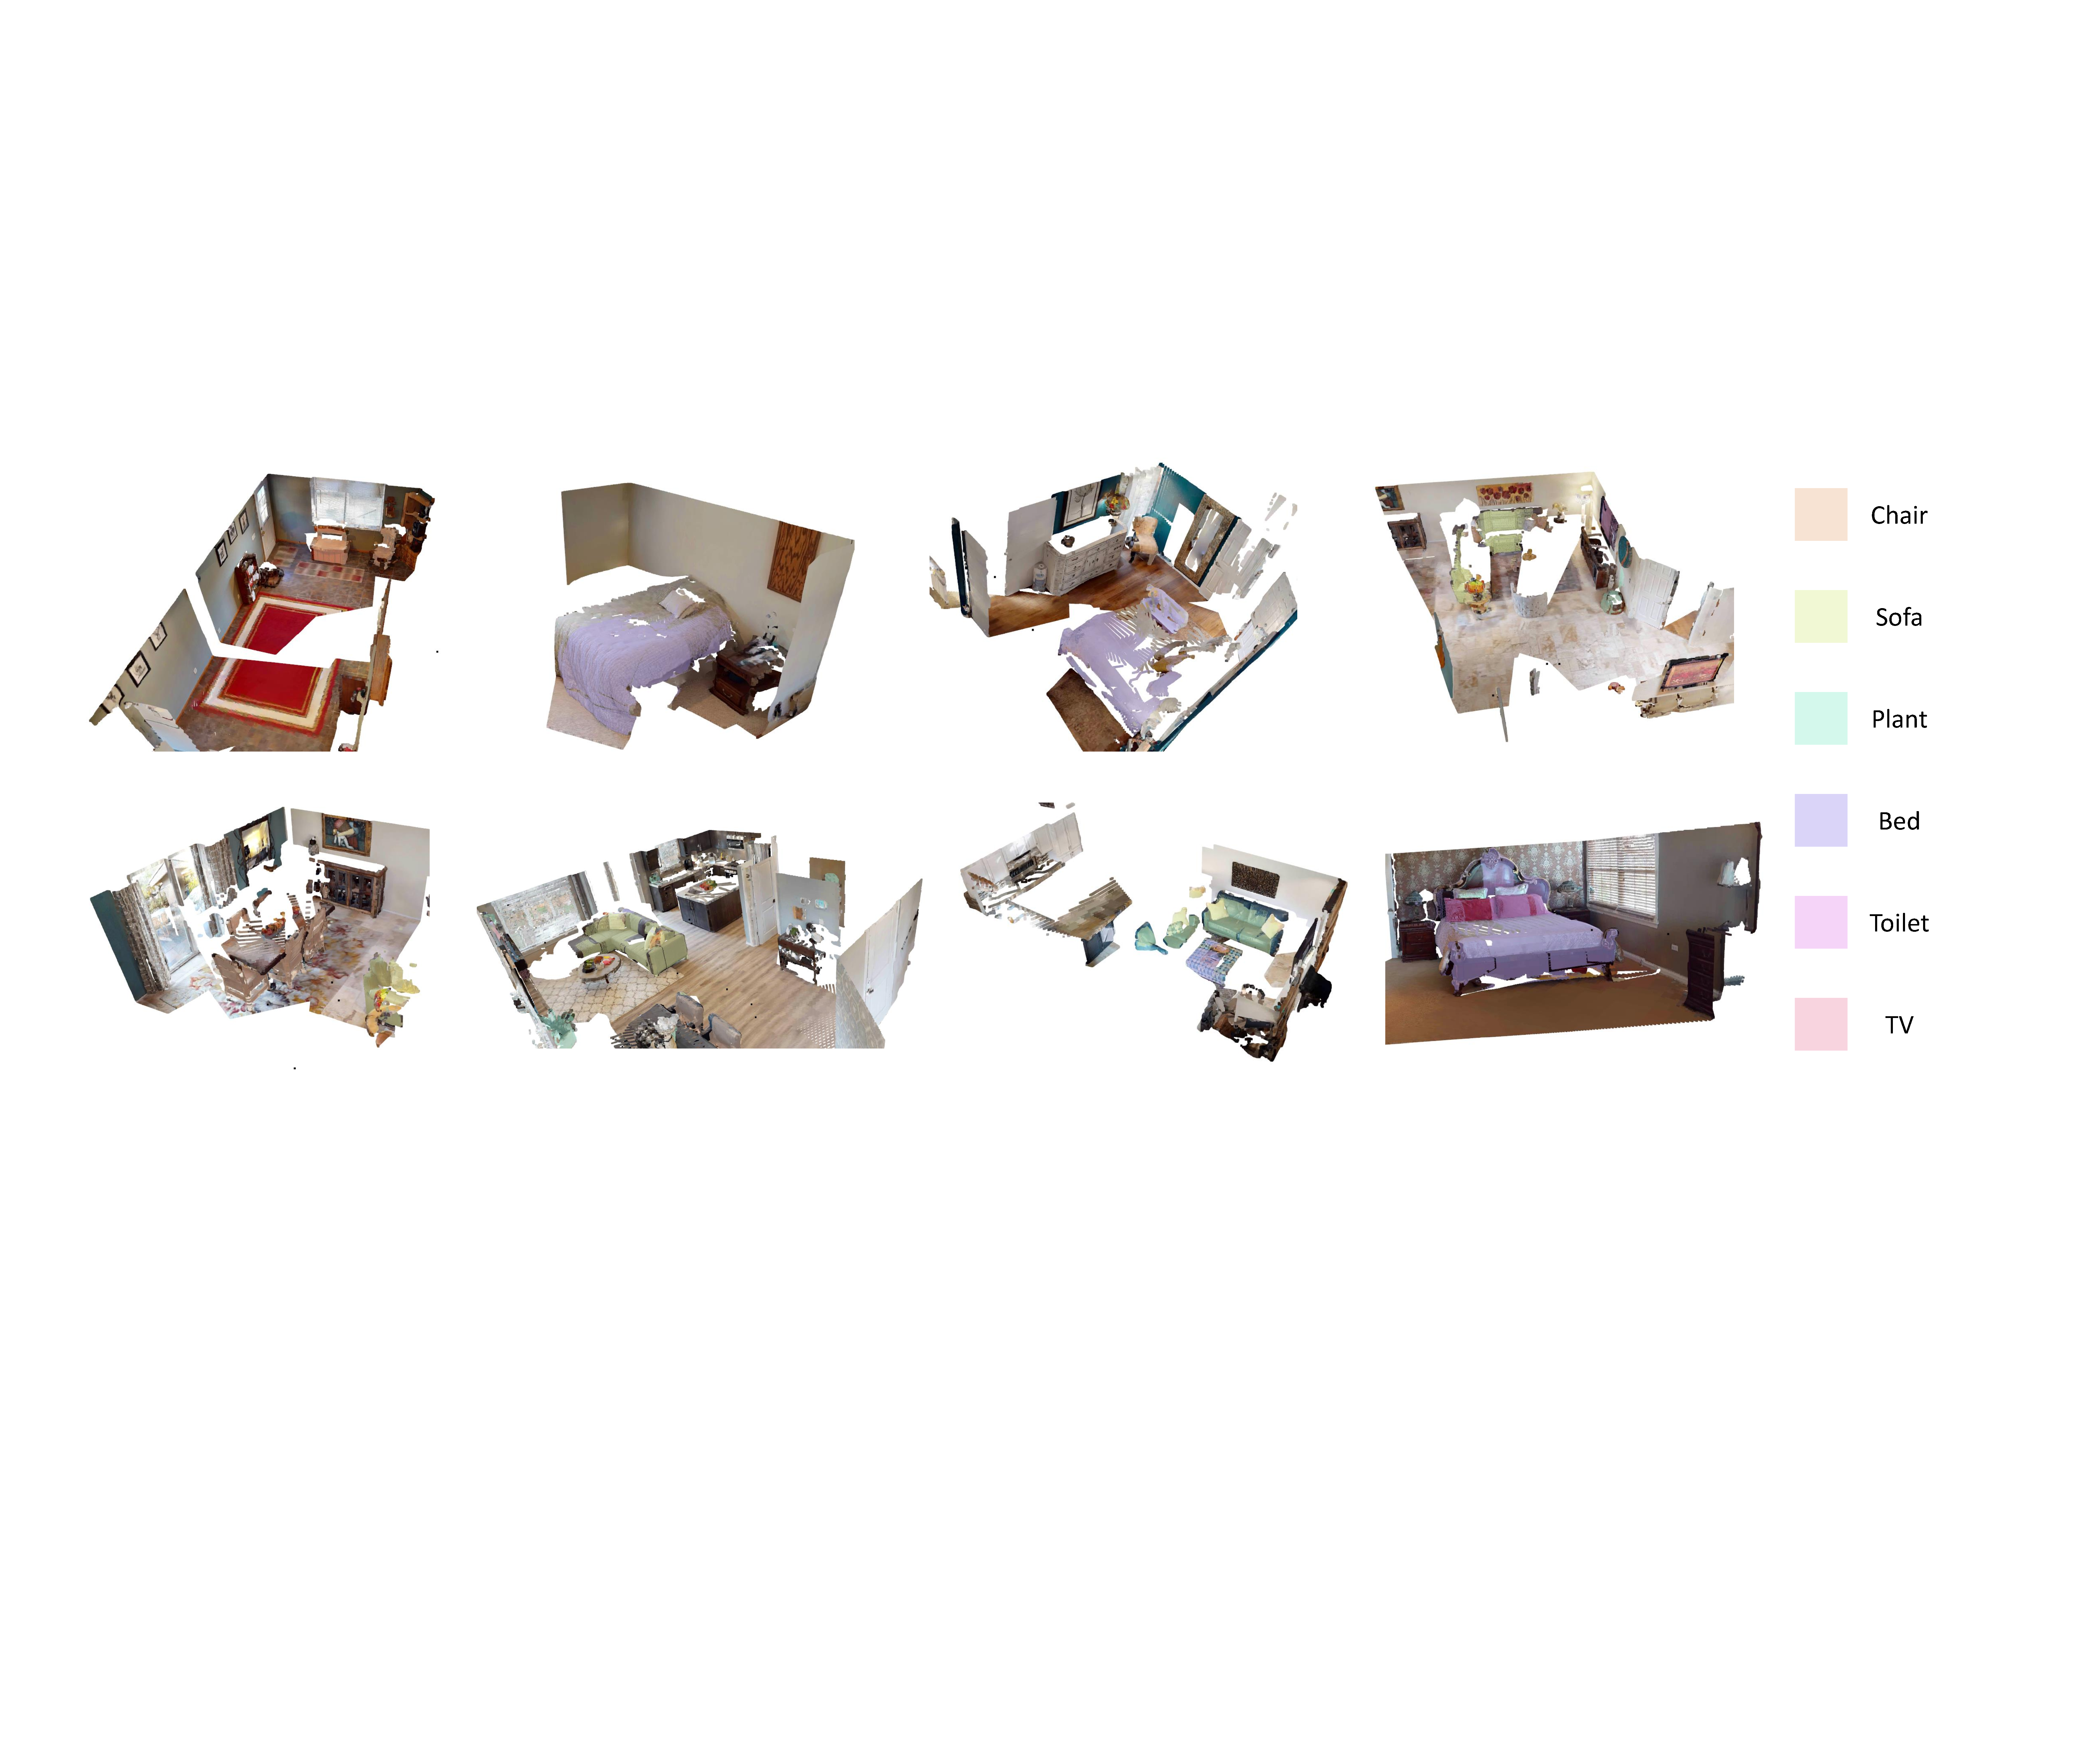
\includegraphics[width=0.95\linewidth]{pics/supp_gauss.pdf}
  \caption{语义高斯可视化结果。
  }
  \vspace{-6pt}
  \label{fig:vis_gauss}
\end{figure*}


我们从预处理和智能体-环境交互两个角度分析了我们方法的时间效率。在我们的方法中，"预处理"指的是给定语义高斯地图后，匹配和定位目标物体的过程。后者则比较了我们的方法与各种其他方法的运行时帧率。


在地图中高效定位目标物体对我们的方法至关重要，我们利用渲染结果来匹配和定位目标物体。为了降低在每个可导航视点比较所有可能观测的计算成本，我们引入了语义高斯。该技术将物体实例按其对应的语义标签进行分组。这种优化通过将比较限制在每个实例的几个描述性渲染图上，显著缩小了搜索空间。例如，在\texttt{CrMo8WxCyVb}场景中，可导航区域量化为$54.03 m^2$。该空间可离散化为约54个正方形，每个面积为$1 m^2$。智能体位于每个正方形内时，可以从12个不同的视角观察周围环境，覆盖完整的$360^\circ$，每个视角跨度$30^\circ$。因此，该单层的原始搜索空间将包含$12 \times 54 = 648$个潜在观测。通过应用基于语义标签的分组策略，搜索空间被大幅缩小。我们统计了\texttt{CrMo8WxCyVb}场景中不同类别的物体实例数量，如\Cref{tab:time}所示。为了定位一把"椅子"——假设我们从三个独特的视角渲染每个物体实例——最终的搜索空间减少到仅$3 \times 11 = 33$个观测。我们渲染单个实例的三个观测以确保渲染质量，这只有在新视角与训练视图大部分重叠时才能实现。这种优化带来了时间效率的显著提升。

\begin{figure*}
  \centering
  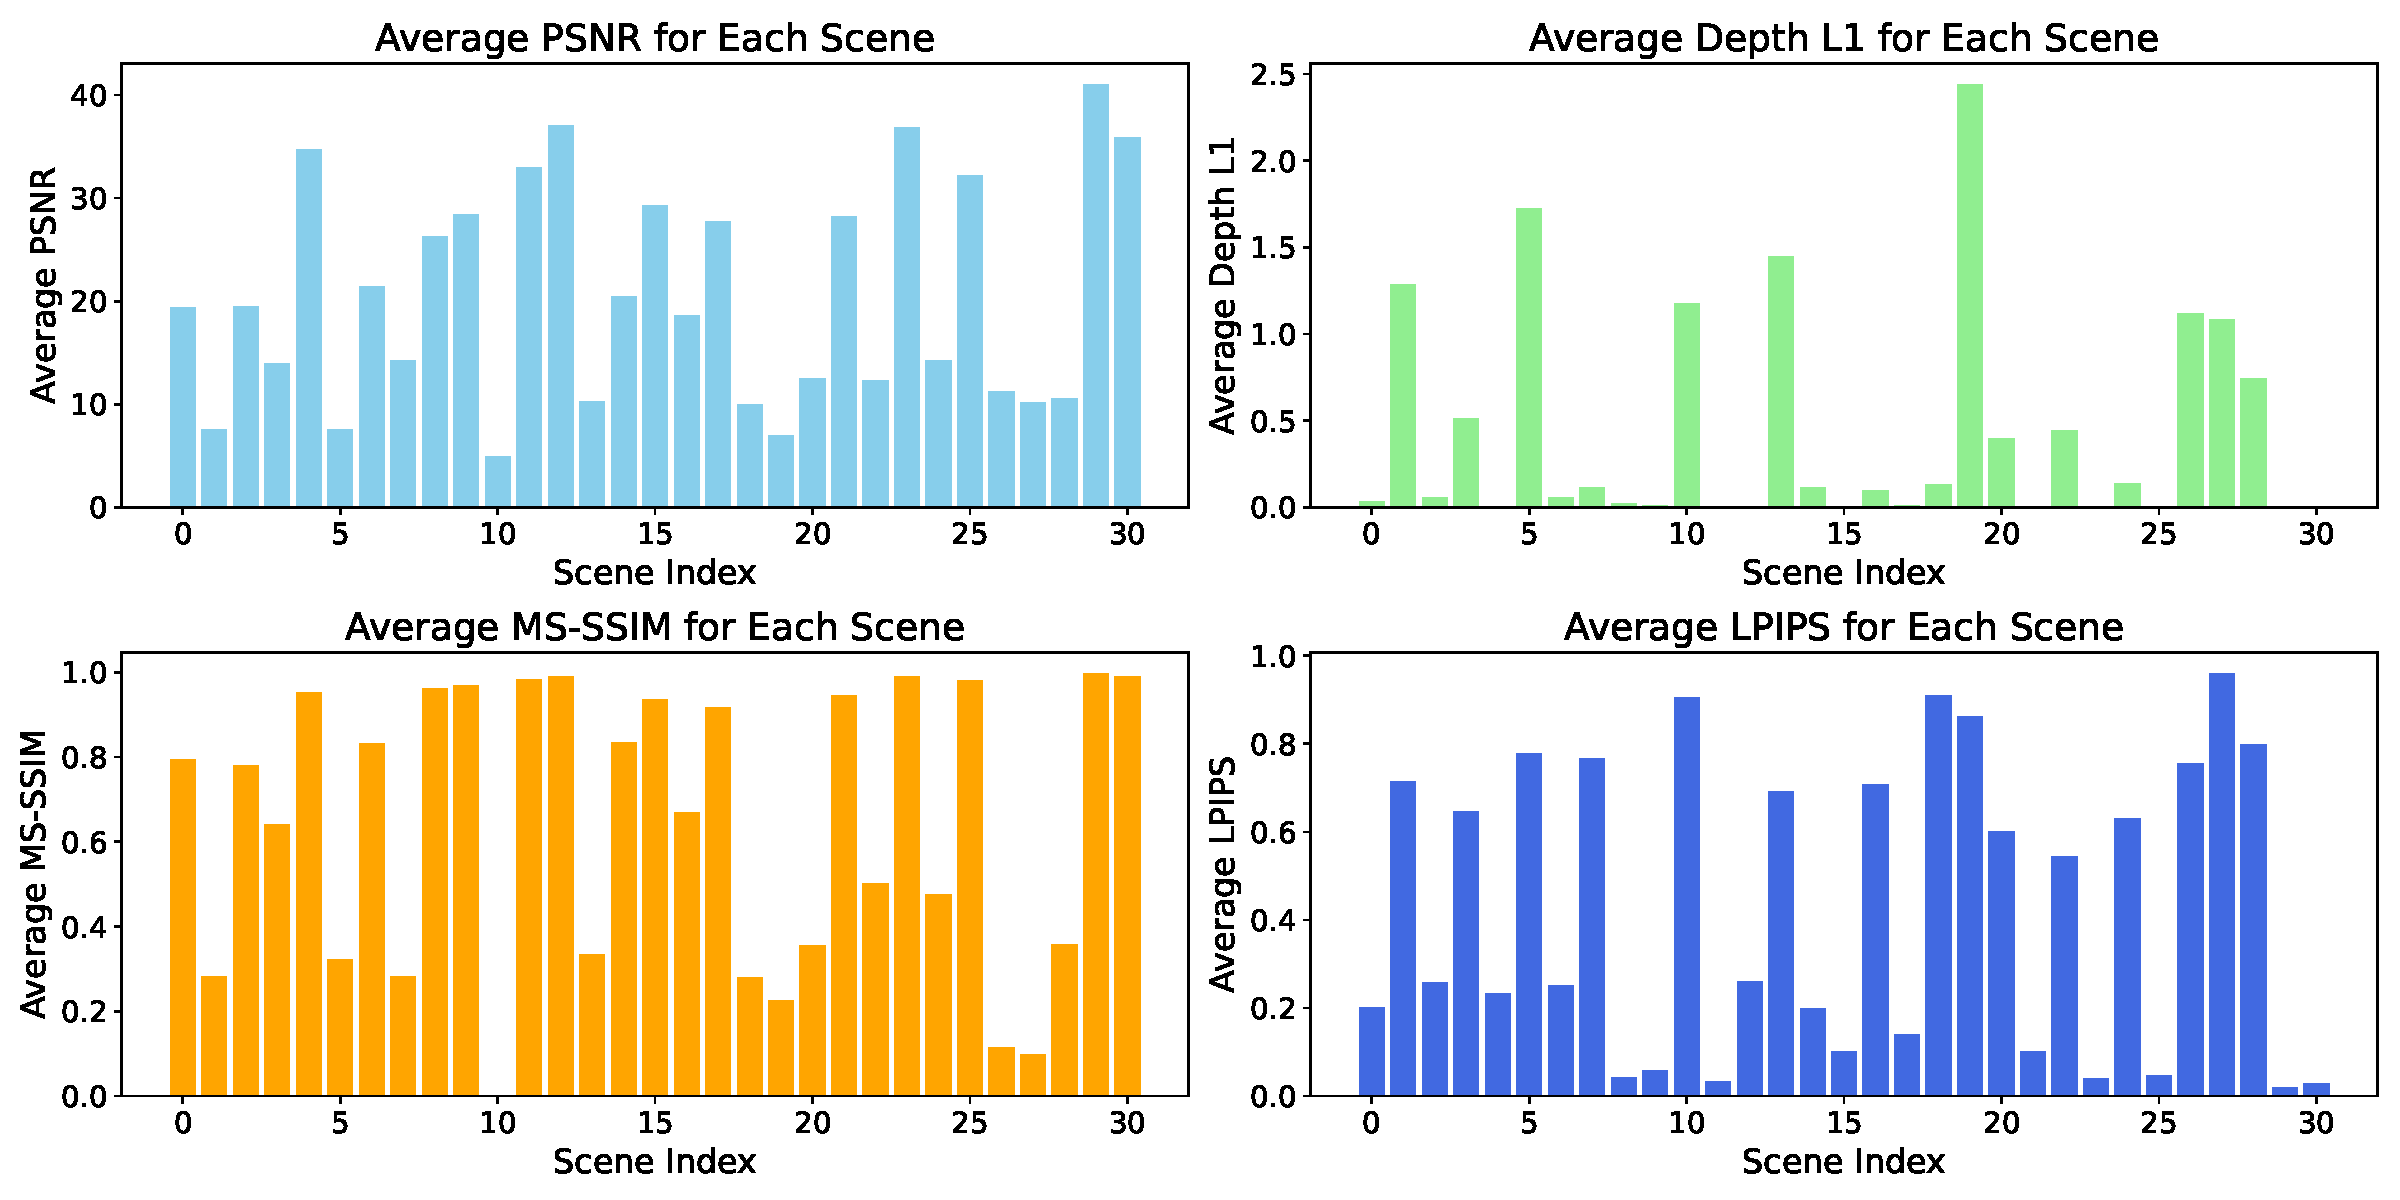
\includegraphics[width=0.99\linewidth]{pics/gauss.pdf}
  \caption{我们的语义高斯构建方法在HM3D验证数据集上的渲染质量。x轴表示不同的场景索引及其对应的楼层高度。
  }
  \vspace{-4pt}
  \label{fig:gauss_results}
\end{figure*}

\begin{figure*}
  \centering
  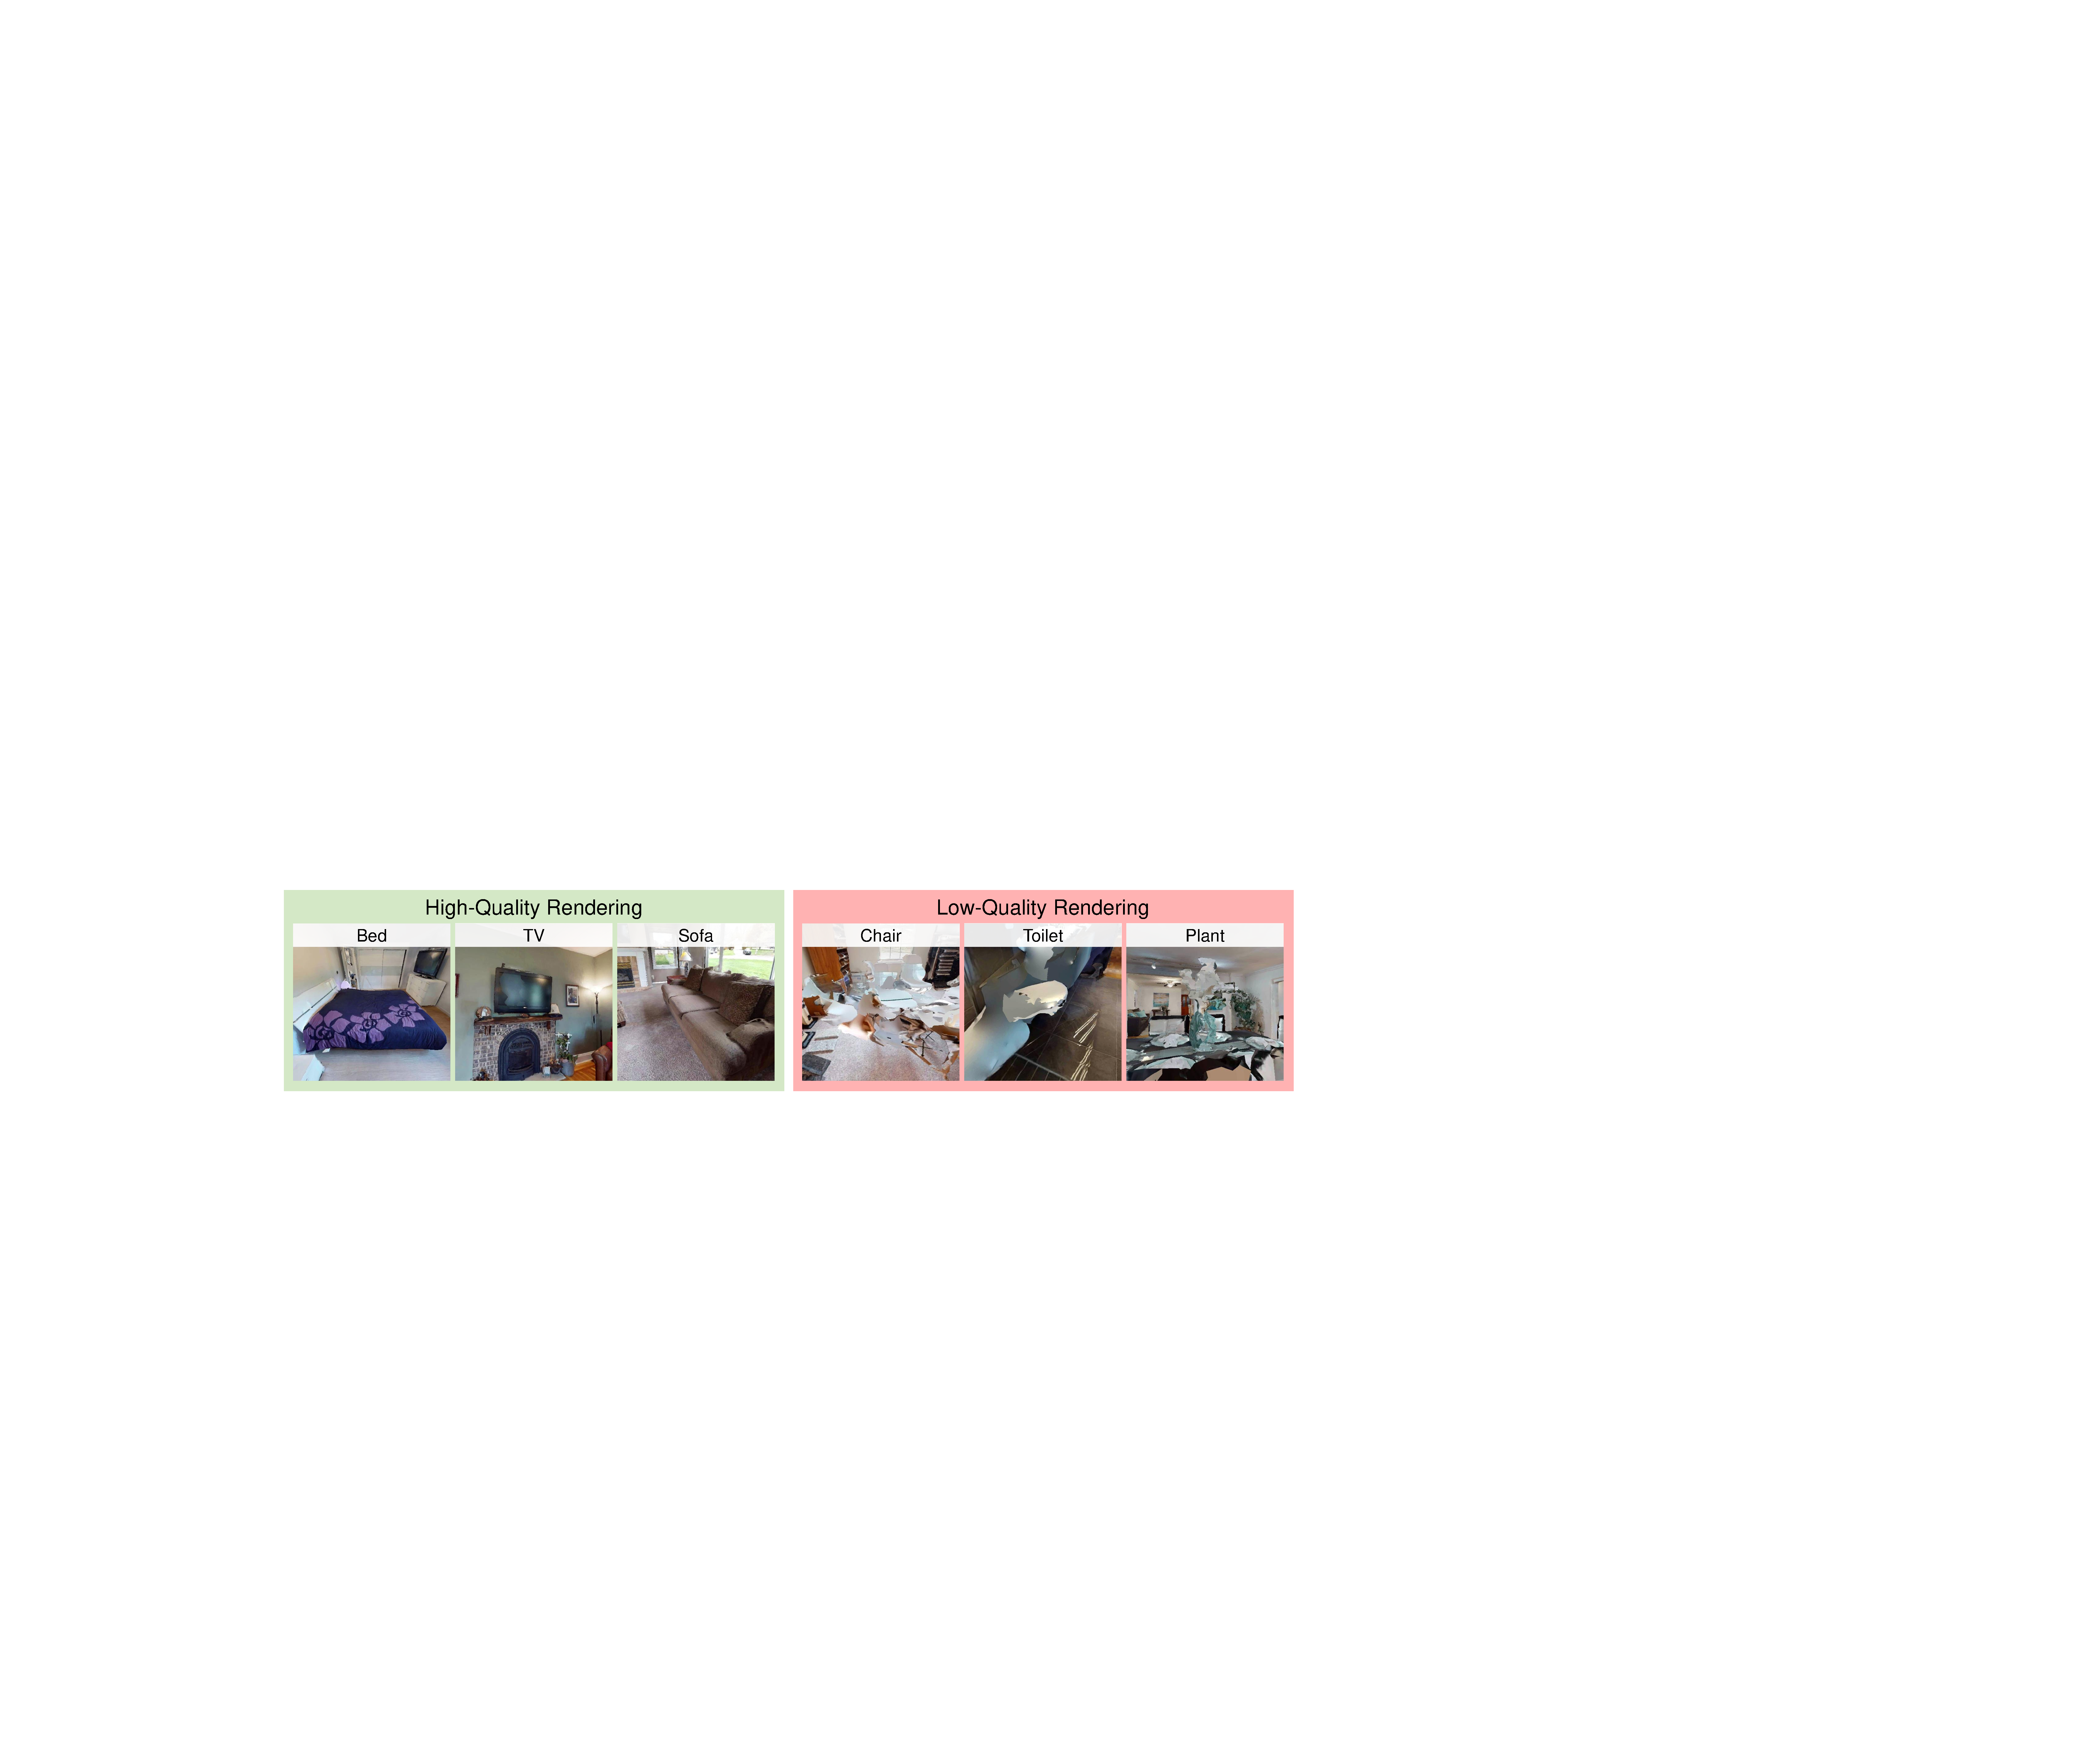
\includegraphics[width=0.99\linewidth]{pics/bad_render.pdf}
  \caption{使用Habitat仿真器\cite{szot2022habitat}从HM3D\cite{yadav2023habitat}场景数据集渲染的观测图像。
  }
  \vspace{-16pt}
  \label{fig:bad_render}
\end{figure*}

我们还在单个Habitat环境中使用NVIDIA GeForce RTX 3090 GPU和10个CPU核心比较了不同方法的运行时帧率。如\Cref{fig:framerate}所示，我们的方法保持了超过20 FPS的高效率，同时在所有对比方法中取得了最高的SPL。为了实现更高的运行速度，GaussNav将语义高斯地图投影得到二维栅格地图。利用"预处理"阶段预测的目标位置，我们然后使用快速行进法(FMM)进行路径规划。我们的方法在速度上优于各种模块化方法的原因是，我们在导航过程中不依赖语义分割\cite{krantz2023navigating, lei2024instanceaware}、局部特征匹配\cite{krantz2023navigating, lei2024instanceaware}或切换模块\cite{lei2024instanceaware}等额外组件。这种简化使GaussNav能够更高效地运行。我们还提供了GaussNav导航至目标物体实例的定性示例，如\Cref{fig:qualitive_result}所示。



\subsection{错误分析}

所提模型的性能仍远非完美。我们希望了解错误模式以便未来改进。我们的分析确定了两个错误来源：第一个是模型无法从实例渲染图中一致地匹配目标，第二个是目标定位不准确。为了量化这些错误来源的影响，我们使用真实值匹配模块和精确的目标定位对模型进行了评估。第一个意味着智能体可以从候选观测中正确识别目标，第二个意味着智能体直接获得真实值目标位置。配备真实值匹配模块的变体（\Cref{tab:ablations}中的\textbf{GaussNav w. GT Match}）表明，成功率可以提高约0.127（\Cref{tab:ablations}第5和第6行）。此外，当模型同时配备真实值匹配和目标定位时，记为\textbf{GaussNav w. GT Goal Localization}，我们观察到成功率从0.850提高到0.946，如\Cref{tab:ablations}第6和第7行所示。第一个错误来源的改进可以通过开发更鲁棒的重识别算法来实现。至于第二个来源，更精确的定位策略可能会产生更好的结果。这些见解不仅突出了模型当前的不足，还为后续的改进工作指明了方向。

\vspace{-3pt}


\subsection{高斯构建结果}



如\Cref{fig:vis_gauss}所示，我们提供了语义高斯的可视化结果。这些示例证明了我们的语义高斯表示在各种场景中的有效性。通过展示更广泛的结果，我们旨在说明我们的方法在处理各种场景复杂度和物体组合方面的鲁棒性和适用性。

在\Cref{fig:gauss_results}中，我们对语义高斯构建方法在HM3D验证数据集\cite{yadav2023habitat}上产生的渲染质量进行了定量评估。为了符合IIN任务\cite{krantz2022instancespecific}的约束，我们将HM3D中的每个场景划分为独立的楼层，并限制智能体在单个楼层内移动，因为IIN任务\cite{krantz2022instancespecific}本身确保智能体的起始位置和目标位置在同一楼层。

为了定量分析\Cref{fig:gauss_results}中的结果，我们观察到渲染结果呈现出两极分化的趋势。例如，在索引为29和30的场景中，渲染图像达到了高达40的PSNR和接近零的深度渲染误差。然而，场景10的渲染性能不佳。我们假设不同场景之间渲染质量的这种两极分化可归因于仿真与现实之间的差异。这在\Cref{fig:bad_render}中很明显，其中使用Habitat仿真器从HM3D数据集渲染的一些图像显示出低保真度，特别是在高纹理环境中。在这种复杂环境中进行高质量重建是困难的，而使用次优渲染图作为三维环境重建的基础会进一步降低最终输出的质量。鉴于此，对于重建质量较差的场景，我们保持一致性，使用原始训练视图，而不是尝试渲染可能导致质量下降的新视图。